%!TEX root = ../Thesis.tex
%! Author = PR
%! Date = 27.05.2020


\section{Projekt-Architektur}

In \cref{fig:root-ordner} ist die grobe Ordnerstruktur des Quellcodes dargestellt.

\begin{figure}[hbt]
    \centering
    \begin{minipage}[t]{1\textwidth}
        \caption{Grobe Ordnerstruktur}
        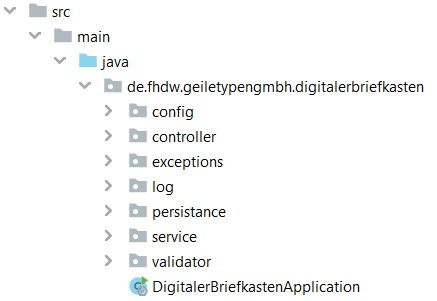
\includegraphics[width=1\textwidth]{img/Projekt-root-ordner.png}\\
        \source{Eigene Darstellung}
        \label{fig:root-ordner}
    \end{minipage}
\end{figure}

In dem Projektordner befinden sich der Unterordner src/main/java/de/fhdw/geiletypengmbh/digitalerbriefkasten. In diesem
befindet sich der erstellte Quelltext. Die Unterordner (Packages) dessen werden folgend grob erklärt.
\begin{itemize}
    \item config
    \subitem Hierin ist die SecurityConfig der Anwendung enthalten.
    \item controller
    \subitem Hierin liegen die Controller. Diese stellen die erreichbaren Endpunkte für die Benutzeroberfläche sowie die REST-API zur Verfügung.
    \item exceptions
    \subitem Hierin sind eigene Exceptions. Diese werden an die Benutzeroberfläche im Fehlerfall weitergeleitet. Ein Beispiel dafür ist die "IdeaNotFoundException".
    \item log
    \subitem Hierin liegen alle Klassen, die zum Logging von Ereignissen dienen.
    \item persistance
    \subitem Das Package persistance dient zum Speichern der Daten (Objekte bzw. Entities) in der Datenbank. Es ist untergliedert
    in die packages
    \begin{itemize}
        \item model
        \subitem Hierin liegen die Datenklassen (Entities). Sie entsprechen dem ER-Diagramm.
        \item repo
        \subitem Hierin liegen die Repositories. Sie dienen zum Lesen, Schreiben, etc. der Datenklassen in die Datenbank.
    \end{itemize}
    \item service
    \subitem Hierin liegen die Services. Sie dienen als Abstraktionsschicht über den Repositories. Damit kann zusätzliche Logik z.B. vor dem Speichern einer Entität implementiert werden. Auch Hilfsmethoden befinden sich in den Services.
    \item validator
    \subitem Hierin liegt die Validationsklasse für die Benutzerstellung. Sie enthält Prüfungen, wie z.B. ob das Passwort lang genug ist.
\end{itemize}
Darüber hinaus befindet sich in dem Package noch die Hauptklasse der Anwendung DigitalerBriefkastenApplication, durch welche sie gestartet wird.
\newline
Neben src/main/java existiert auch der Ordner src/main/resources. In diesem sind die Komponenten für die Weboberfläche der Anwendung enhalten.
In \cref{fig:resources-ordner} wird die Struktur von resources dargestellt.

\begin{figure}[H]
    \centering
    \begin{minipage}[H]{1\textwidth}
        \caption{Grobe Ordnerstruktur}
        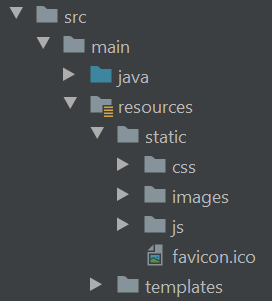
\includegraphics[width=0.5\textwidth]{img/resources-ordner.png}\\
        \source{Eigene Darstellung}
        \label{fig:resources-ordner}
    \end{minipage}
\end{figure}


Der Unterordner static beinhaltet css-, Bild- und JavaScript-Dateien. In Templates befinden sich die HTML Dateien.

